\chapter{绪论}

\section{研究背景}
\indent
文化兴则国运兴,文化强则民族强。文化是国家的灵魂,民族的血液。2024年7月,党的二十届三中全会胜利完会,全会审议通过的《中共中央关于进一步全面深化改革、推进中国式现代化的决定》 ~\cite{xjptheory1} 中特别指出,要优化文化产品供给机制,激发全民族文化创新创造活力,这其中有两个着力点,就是强化创作导向、借力技术创新。为了更好更牢地以文化为重要支点推动经济高质量发展,不断实现文化与经济交融互动、融合发展,我们需要积极推进以文兴业、科技赋能,大力发展以“文化+创意”“文化+科技”为主要特征的文化创意产业,成为有效应对发展挑战、培育新的经济增长点的突破口~\cite{theory2} 。尽管文创领域发展一片良好,但现阶段还是存在一些问题:
\newline \indent
(1)文创产品的质量不够高,难以满足人们日益增长的审美需求。
\newline \indent
(2)文创开发的效率较低下,对于某一难以在短时间内产出多种相关的创作成果,难以在快速波动的市场中抓住商业机会。
\newline \indent
为了更好地聚焦于两个着力点,强化文化数字产品的创作能力,有效提升我国文化创作水平,我们可以利用风格迁移技术。风格迁移技术是一种强大的技术,通过往特定场景中引入风格化图像的风格特征并融合处理,创造出新的风格化的艺术场景。其中二维图像风格迁移可以用在广告、设计和媒体等领域,通过改变图像的外观和装饰,使其更加引人注目和独特。三维风格迁移是将一个场景的风格提取并且应用到另一个场景的三维模型上,可以为虚拟现实、游戏开发和电影制作等领域注入新动能,推动文化产业的创新创优,丰富人民的文化生活。
\newline \indent
经过多年的发展,风格迁移技术得到了长足进步,但是还是存在以下问题~\cite{jing2019neural}:
\newline \indent
(1)图像的风格纹理特征不够细致。现有的图像的任意风格迁移算法不能在生成无伪影的高质量图像的同时充分兼顾如颜色,笔触,色调,纹理等艺术特征,导致。现有的内容和风格特征之间对齐的方法还需要进一步完善,以保障更高质量的特征混合。同时现有的风格特征使用VGG~\cite{simonyan2014very}编码器进行提取,它更适合分类任务的特征处理,而在关注颜色,笔触、纹理等艺术特征方面还可以进一步优化。
\newline \indent
(2)3D场景风格迁移技术的性能权衡问题:现有的3D场景迁移模型多少在以下方面有一些不足:多视角一致性不够、对任意一个新的风格图片都需要重新进行风格化训练、训练推理速度较慢等、在面对更多的约束和挑战下,场景的风格化质量不佳等。有的模型结构过于复杂对设备要求较高,而且将它们应用到现实中充满各种物体的3D环境中存在较大不足。


% \begin{enumerate}
%     \item 删除根目录的 ``.latexmkrc'' 文件,否则编译失败且不报任何错误
%     \item 字体有版权所以本模板不能附带字体,请务必手动上传字体文件,并在各个专业模板下手动指定字体。
%         具体方法参照 GitHub 主页的说明。
% \end{enumerate}


\section{研究目标及内容}
近年来,随着经济科技的快速发展,人们对于文化艺术产品的要求也越来越高。艺术风格迁移作为一种通过将风格注入到内容载体中来创造视觉上有吸引力的图像的方法越来越受欢迎。但是现有的2D风格迁移方法无法在较好地考虑风格的颜色,笔触,色调,纹理等艺术特征地同时做到无伪影地风格迁移。与此同时,现有的3D场景风格迁移技术,均不同程度地存在多视角一致性不够、无法做到零样本迁移、对算力要求较高、训练推理速度较慢等。因此,本文的研究目标是针对设计一个新的2D图像任意风格迁移算法,并提出一个支持不同风格迁移方法的零样本3D场景快速风格迁移框架。具体来说,本文具体的研究内容主要包括以下两个方面:
\newline \indent
(1)提出一种基于风格一致性实例归一化和对比学习的2D图像任意风格迁移算法。它由三个模块构成其中风格一致性实例归一化 (SCIN)模块用来提供全局风格信息,该模块使用一个transformer模块作为一个全局的风格提取器,从风格图中提取长程的风格信息,实现从分布上将内容特征与风格特征对齐;基于实例的对比学习(ICL)方法通过图像的潜码空间约束图像的像素级内容,用来学习风格化到风格化的关系、提高风格化质量;并且我们提出了一个新的感知编码器(PE),它可以捕获风格信息,避免模型过多关注风格图像的显著分类特征。   
\newline \indent
(2)提出一种基于超网络和可变3D高斯点的零样本三维场景风格迁移框架。该框架支持通过即插即用的方式使用任意的2D风格迁移方法作为3D场景风格迁移的监督,并且使用3DGS的方法作为3D建模表示的方法。使用编码器提取风格图的特征,将提取后的特征通过特别训练的超网络和变形网络,超网络输出对变形网络的控制权重,变形网络对3DGS的较后进行致密化操作的部分高斯点的颜色属性表达进行一些调整,在保证快速训练快速渲染的同时实现良好的多视角一致性。
\newline \indent	
本文提出的方法为场景的任意风格迁移工作提供了新的思路和方向,给相关工作提供了一种新的框架和思路,更好地促进相关需求的高水平实现。

\section{本文组织架构}
本文深入探讨了风格迁移领域的各种方法,对其原理、优势和局限性进行了详尽的分析。在此基础上,文章提出了一种创新的架构和一种创新的任意图像风格迁移算法,旨在解决现有风格迁移技术中存在的问题。文章还通过实验验证了新架构的有效性,并通过与其他方法的比较,展示了其在风格迁移任务中的优越性能。全文内容如下:
\par 第一章为绪论,简述了风格迁移的意义和必要性,同时简要介绍了当前风格迁移主要的方法,并指出当前风格迁移领域存在的一些问题,在此基础上阐明了本文的研究目标与内容。 
\par 第二章是本文相关技术的综述,介绍了现有的2D风格迁移算法的发展历程和现状,同时分析了典型方法的优缺点;也介绍了3D风格迁移算法的技术路线和优缺点;还介绍了对比学习和蒸馏学习方法的基本原理,为后续的章节奠定了理论基础。
\par 第三章提出了一种基于风格一致性实例归一化和对比学习的2D图像任意风格迁移算法,对该算法的总体架构、损失函数和训练过程作了详细的介绍,并通过丰富的对比实验和消融实验验证了算法的效果。
\par 第四章提出了一种基于超网络和可变3D高斯点的零样本三维场景风格迁移框架,对该算法的模型各部分及损失函数、训练过程作了详细的介绍,并通过实验验证了该框架的有效性。
\par 第五章总结了本文的工作成果,肯定了一些创新之处,并且对于存在的一些不足进行了阐述,同时对未来工作进行了展望。

\section{本章小结}
本章首先说明了风格迁移技术研究对于国家文化强国战略、对于文艺工作者的积极意义,然后分别阐述了风格迁移技术的应用场景和2D图像风格迁移、3D场景风格迁移的发展概述,指出现存的风格迁移算法在特定领域的不足,从而引出本课题的研究目标和内容。最后说明了全文的组织架构。  

\chapter{相关技术介绍}
风格迁移技术是通过一定的技术手段,把某个艺术载体的内容同另一个载体的艺术风格融合在一起,产出具有新的艺术风格且保留原有内容特征的艺术品的一种技术。
按照艺术载体的不同,它可以分为图像(含视频)的风格迁移和三维场景的风格迁移。自从2015年Gatys等人~\cite{gatys2016image}提出使用深度学习的方法进行图像风格迁移以来,图像的风格迁移技术有了长足的发展,
众多使用深度学习的图像风格迁移的方法涌现出来。从分类上可以分为单风格迁移和任意风格迁移两个大类。单风格迁移方法包括基于优化的在线方法和基于前馈网络的离线计算方法~\cite{jing2019neural}。
任意风格迁移主要使用两种手段实现:采用可变参数的归一化方法调整内容特征,或者采用交叉注意融合风格属性和内容属性。
基于深度学习的场景风格迁移主要采用某些方式对场景进行建模,并且把风格的特征通过某些手段融入到建模之中,并且通过渲染显示出场景的风格化结果。
当前常用的效果较好的方法按照建模的表示方式不同可以分为基于点云和体素建模的场景风格迁移、基于神经辐射场(NeRF)~\cite{mildenhall2021nerf}建模的场景风格迁移和基于3D高斯飞溅(3DGS)建模的场景风格迁移。
下面将对二维图像的神经风格迁移算法、三维场景的神经风格迁移算法研究现状和对比学习的理论进行一个介绍。
\section{二维图像神经风格迁移算法介绍}
\subsection{单风格迁移方法}
单风格迁移方法的特点就是模型每次训练和运行完毕只能处理一张内容图和一张风格图并生成一个结果。从技术上看可以分为基于优化的在线方法和基于前馈网络的离线计算方法~\cite{jing2019neural}。下面将对这两类进行分别介绍。

\paragraph{基于优化的在线方法}
基于优化的在线方法主要通过一些方式提取出内容图像和风格图像的特征,并且迭代地优化生成图像,以使其被提取的特征能够满足内容约束和风格约束。
Gatys 等人~\cite{gatys2016image,gatys2017controlling}首先提出利用VGG-19~\cite{simonyan2014very}的部分中间层的特征输出来实现对给定照片的内容特征和给定艺术图像的风格特征的提取,
并且通过限制目标图像和内容图像的特征差异来实现风格化的内容保持、通过限制目标图像和风格图像的统计特征差异(即Gram矩阵)来实现风格的重建,从而得到风格化后的图像。
该方法是不需要训练的,能够成功地生成具有给定艺术品外观的风格化图像。然而,由于VGG-19特定层提取出来的图像特征不可避免地会丢失一些底层信息,
该算法在风格化过程中不能很好地保持精细结构和细节的连贯性。此外,它也未考虑笔触等属性的变化。
为了优化这些问题,有一部分研究者对于统计特征差异的限制这一方面进行了一些研究,取得了一些成效,提出了一些其他有效的风格的统计表示,
它们是从基于Gram矩阵的表示派生出来的。Li等人~\cite{li2017demystifying}通过从领域适应的角度出发来看待风格迁移问题,提出来了通过最小化分布间的差异来建立源领域样本和目标领域样本间的联系,
通常使用最大平均差(Maximum Mean Discrepancy,MMD)衡量两个分布间的差异,并且证明了在一对风格和风格化图像之间匹配基于Gram矩阵的样式表示同使用最小化二次多项式核的MMD是本质上等价的,
且可以使用其他的核函数来实现其他的风格化应用。另外,Risser 等人~\cite{risser2017stable}引入了直方图损失函数(Histogram loss),用于缓解Gram矩阵的不稳定训练问题。

\paragraph{基于前馈网络的离线计算方法}
基于前馈网络的离线计算方法与基于优化的在线方法相比,有着指极大的效率优势。
考虑到优化方法需要不断地进行迭代,且在进行风格迁移的时候迭代计算量很大、速度很慢这一问题,Ulyanov 等人~\cite{ulyanov2016texture}提出来训练一个神经网络,在训练的时候承担这一计算任务,
并且在推理的时候能够通过简单的网络前向传播过程来更快速地实现风格迁移,这就是最初的基于前馈网络的方法。
在这一思路上,Johnson 等人~\cite{johnson2016perceptual}改变了一部分网络的架构,并且提出了一个很有用的损失即感知损失(Perceptual loss),
这个损失能够有效度量生成的图和原图在人眼感知方面的差异,为未来的风格迁移任务所广泛使用。
随后,为了更进一步改进风格化质量,并且为了增加一些纹理多样性,Ulyanov 等人~\cite{ulyanov2017improved}进一步提出,
简单地将归一化(Normalization)操作应用于每一张图像而不是整批(Batch Normalization)可以较显著地提高规范化质量和网络收敛速度。
同时Ulyanov等人也提出了让生成器遵循一致地Julesz ensemble采样~\cite{zhu2000exploring}的方法以增加纹理的多样性。
同时,Li等人~\cite{li2016precomputed}提出乐基于马尔可夫随机场(Markov Random Field,MRF)的快速单风格迁移方法,他们通过对抗训练训练了一个基于片的非参数马尔可夫前馈网络来取得更好的连贯纹理。

\subsection{任意风格的快速迁移方法}
前述的风格快速迁移方法对于每个新的风格图,都需要重新训练,对于需要频繁使用多种风格进行迁移操作的用户的体验还是不够友好,因此需要研究任意风格的快速迁移方法,其显著特点就是一次训练就可以适用于任何风格图的推理应用。从特征的处理方式来看可以分为以下两类:采用可变参数的归一化调整内容特征和采用交叉注意融合风格属性和内容属性。下面分别进行介绍。
\paragraph{采用可变参数的归一化调整内容特征的方法}
本系列方法的理论核心是归一化在风格迁移网络中的作用:为了对风格进行建模,在对每个特定风格进行归一化后专门对缩放和偏置参数进行仿射变换就足够了。
这就是Dumoulin等人~\cite{dumoulin2016learned,ghiasi2017exploring}提出的条件实例归一化方法(Conditional Instance Normalization,CIN),它是一种简单但是强大的方法,
在IN的基础上引入条件参数,用于在图像风格迁移中控制生成图像风格。随后,Huang等人~\cite{huang2017arbitrary}提出在CIN的方法上改进为自适应实例归一化(Adaptive Instance Normalization,AdaIN),
这也是一种简洁而强大的网络。它在通道层面上用输入图像和想要变成的目标风格图像的均值和方差取代了CIN中的条件参数,从而能够简单地调整统计特征的均值和方差。
AdaIN的训练流程是:先用VGG编码器提取内容图和风格图的特征,然后在AdaIN模块进行的操作,然后用同编码器对称的解码器网络将特征还原为图像,
然后将还原的图像再输入到编码器提取特征,计算损失函数。编码器的参数在训练过程中是不更新的,训练的目的是为了得到一个好的解码器。
\par Li等人~\cite{li2017universal}的思路同AdaIN相似,但是由于观察到白化变换可以去除风格相关信息并保留内容结构,他们将编码器和解码器中的AdaIN层替换
为一对白化和颜色变换(Whitening and Coloring Transformation,WCT),然后,通过应用着色变换,将风格特征中包含的风格模式合并到过滤后的内容表示中,
并且可以通过解码转换后的特征来获得风格化的结果。但是上述方法的缺点是它们对全局特征进行的归一化处理使得网络难以合成具有丰富细节和局部结构的复杂风格模式。
An等人~\cite{an2021artflow}提出由可逆神经流和无偏特征迁移模块组成的ArtFlow来防止通用风格迁移过程中的内容泄漏问题。
\par 除此之外,其他人也从不同的思路对方法进行优化和创新。Li等人~\cite{li2019learning}提出的LST,可以学习以数据驱动的方式转换特征矩阵的能力。
该算法高效而灵活,可以用相同的自编码网络迁移不同层次的风格。为了更好地融合内容和风格特征,Wu等人~\cite{wu2022ccpl}提出了简单协方差变换(SCT)
来有效地将内容特征的二阶统计量和风格特征对齐以用于通用风格迁移。并且还提出了对比一致性保持损失(Contrastive Coherence Preserving Loss,CCPL)。
CCPL可以在风格转换过程中保持较高的风格化质量和内容源的连贯性。此外,它具有邻域调节机制,大大减少了局部失真,显著提高了视觉质量。
但是这些方法依然不能生成具有颜色、笔画、色调、纹理等艺术元素的高质量的图像。

\paragraph{采用交叉注意融合风格属性和内容属性的方法}
随着Transformer结构~\cite{vaswani2017attention}的逐渐广泛使用,基于注意力机制的方法也被应用融合内容和风格的属性上来。
比较有代表性的是Park等人~\cite{park2019arbitrary}提出的SANet。它针对的问题是上述方法难以平衡内容结构和风格模式和难以维护全局和局部风格模式的问题。
它在前述方法的整体架构上提出了一种新颖的风格注意力网络,根据内容图片的语义空间分布来高效灵活地融合局部风格模式,
同时还提出了一种新颖的身份损失函数(Identity loss)来保留内容结构并丰富样式模式。
它使用VGG-19编码器的4-1层输出和5-1层输出做注意力计算,并用可学习的相似度核来将内容特征图表示为与其每个位置相似的风格特征的加权和。
这个身份损失函数的作用是计算相同输入图像(内容图像或风格图像)之间的差异,而不涉及风格特征的差异。
\par 在SANet的基础上,Liu等人~\cite{liu2021adaattn}结合SANet和AdaIN的优点,
提出了自适应注意力归一化AdaAttN算法和局部特征损失,以改善任意风格迁移的局部失真问题。
SANet方法由于基于较高层的特征设计注意力机制,忽略了低层次的细节,所以天然地还会存在一些局部失真问题。
该方法加入注意力机制的目的是模型应该更多的关注样式图像中与特征相似的区域。因此提出的AdaAttN方法可以自适应的对每一个点进行注意力归一化,
以实现特征分布的对齐。AdaAttN同AdaIN和SANet在计算上的区别如下\autoref{fig:diff_adain_sanet_adaattn}所示。
\begin{figure}[htbp]
    \centering
    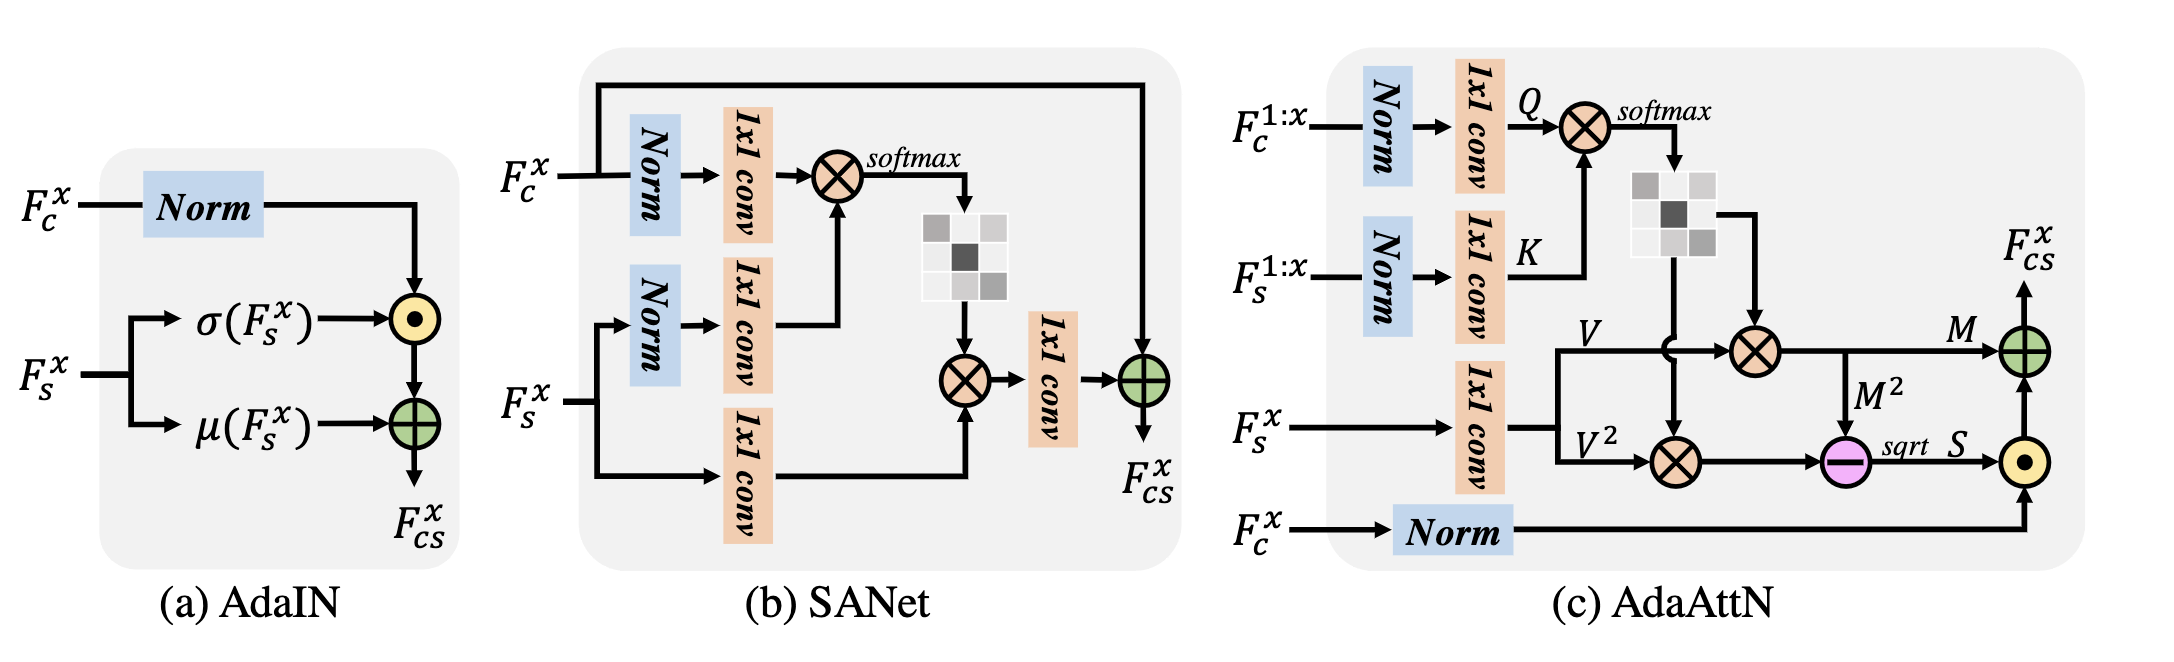
\includegraphics[width=\linewidth]{pics/diff_attn_p1}
    \caption{\label{fig:diff_adain_sanet_adaattn}三种方法在计算上的差别示意图}
\end{figure}

AdaAttN的总体流程如下:首先从浅层到深层计算包含内容和风格特征的注意力图,其中注意力机制被逐层计算用来衡量内容和风格特征之间的相似性。
随后基于注意力图计算风格特征的加权均值和标准差图。最后使用自适应归一化内容特征实现特征分布对齐。
针对SANet的问题,还有一些人对他做出了相应的优化。其中Chen等人~\cite{chen2021artistic}提出一种具有两种对比性损失的内部-外部风格转移方法。
它保留了风格注意力网络,并且利用单个风格图像的内部统计特征来确定风格化图像的颜色和纹理模式,
同时,还利用大规模风格数据集的外部信息来学习人类感知上的风格特征,
这使得风格化图像中的颜色分布和纹理模式更加合理和谐。
同时间,Deng等人~\cite{deng2022stytr2}提出了一种称为 StyTr2 的基于transformer的风格迁移模型。
该框架包括了一个新的感知内容位置编码(Content-Aware Positional Encoding,CAPE),其
中心思想是为图像风格迁移任务引入一种更加灵活和适应性的位置信息编码方式,
保证不同尺度的图像仍然有一致的空间关系。该模型认为风格图像不需要在编码期间严格保持位置关系,而内容图像需要,
故而该模型的风格图像编码器和内容图像编码器的唯一差别在于风格编码器没有应用CAPE。
经过训练以生成具有良好保留结构和输入内容图像细节的风格化结果。Ma等人~\cite{ma2023rast}提出了一种迭代的架构,
从图像修复的角度解决内容泄漏问题。可以通过多次的图像修复操作同时实现内容和风格信息的传输。
他们提出了两个新颖的损失函数--多修复损失和风格差异损失来确保更高的风格迁移质量。

\section{三维场景的风格迁移方法介绍}
近年来,随着科技的发展和人们收入的增加,人们对获取更优良的三维模型的需求也随之水涨船高。
三维的场景不仅可以提供更真实、更具体、更立体的展现形式,还可以使用户获得更加沉浸式的体验和感受。
三维风格迁移技术的核心目标是在保持三维场景结构和多视角一致性的同时,将指定图像的艺术风格自然地应用到三维模型上,
这项技术能够为艺术家和设计师提供强大的工具,使他们能够比较轻松地将特定的艺术风格应用到3D的场景环境中。
三维场景的风格迁移现有的研究基础较为丰富,从场景的表达方式上来看主要可以分为三类:基于显式三维数据表示的风格迁移方法、基于隐式神经辐射场
(Neural Radiance Field,NeRF)表示~\cite{mildenhall2021nerf}的风格迁移方法、基于三维高斯飞溅(3D Gaussian Splatting,3DGS)表示~\cite{kerbl20233d}的风格迁移方法。下面将逐一进行介绍。


\subsection{基于显式三维数据表示的风格迁移方法}
最早的方法是使用点云或者三角形网格来对真实场景进行建模。Huang等人~\cite{huang2021learning}使用VGG-19的编码器提取出模型的特征和风格图像的特征,
并且使用了一种新颖的聚合算法把特征融入,并且使用经过训练的解码器渲染生成新的风格化视图。Mu等人~\cite{mu20223d}的思路同Huang等人相似,
但是使用AdaAttN结合UNet网络进行单图的风格化新视角生成。尹等人~\cite{yin20213dstylenet}提出了3DSTYLENET,
它由两个主要网络组件即几何和纹理风格传输网络组成。首先在一组无纹理形状上预训练3D几何样式传递网络,
在图像数据集上预训练纹理样式传递网络。然后将几何和纹理进行联合优化。 
通过将形状和纹理样式从一个纹理网格转移到另一个纹理网格来创建 3D 网格的新颖几何和纹理变化。
但是这种方法的性能受到几何重建方法本身的质量的限制。随着后来新的高效的几何重建方法被提出,使用显式三维数据用于场景风格迁移的方法也逐渐在性能上不如新方法了。
\subsection{基于隐式神经辐射场表示的风格迁移方法}
相比而言,神经辐射场NeRF的提出很好地改善了几何重建领域的新视图合成质量差、表示方式不灵活、训练较慢等问题,具有重要的意义。
为了更有利于理解,本文拟先对该方法进行一个全面的介绍,然后再介绍基于NeRF表示的风格迁移方法研究现状。


%2.2.2.1
\paragraph{NeRF方法介绍}
NeRF方法由谷歌高级研究科学家Jon Barron在2020年首次提出,是一种基于深度学习的三维场景重建和渲染方法,它通过神经网络模拟场景的连续体积密度和颜色,
从而实现从二维图像数据中恢复出逼真的三维场景。NeRF的核心在于使用一系列从不同角度拍摄的图片来训练一个小型的神经网络,
该网络能够预测从任意视角观看场景时的体积密度和颜色。把物体看作一团可以自发光的粒子,这些粒子具有颜色C,密度σ两个属性。
使用现有的照片对体空间内粒子的密度和颜色进行预测,保存这些信息。在渲染其他视角时,使用这些信息(粒子的密度,颜色)进行推理,就能得到新视角下该场景的照片。NeRF的流程如\autoref{fig:nerf_show}所示:
\par 具体来说,NeRF要解决的问题就两个:
% \par 1. 如何通过现有的照片得到空间中密度与颜色的分布。
% \par 2. 如何利用这些数据,得到任意角度的照片。
\begin{enumerate}
    \item 如何通过现有的照片得到空间中密度与颜色的分布。
    \item 如何利用这些数据,得到任意角度的照片。
\end{enumerate}
\begin{figure}[htbp]
    \centering
    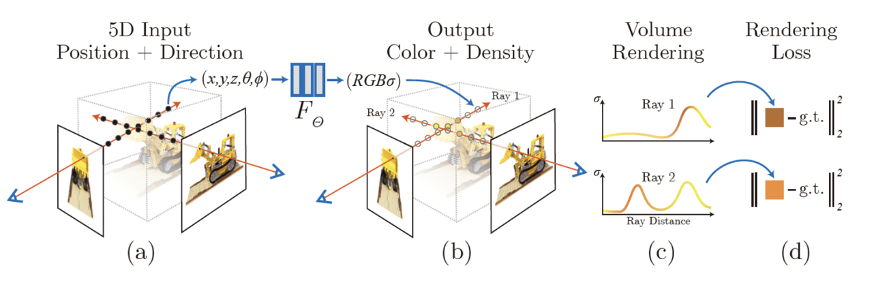
\includegraphics[width=\linewidth]{pics/nerf.png}
    \caption{\label{fig:nerf_show}NeRF方法的流程图}
\end{figure}



对于问题2,可以认为,从某一点看过去,这一点的颜色应该由达到这一点的光线上累积的颜色决定,想象每条光线路径上经过一个个小球到达最终像素上,
最终这些小球以自己的属性参与影响像素的颜色,这一计算可以用\autoref{equ:nerf_color_predict}表示:
% \begin{figure}[htbp]
%     \centering
%     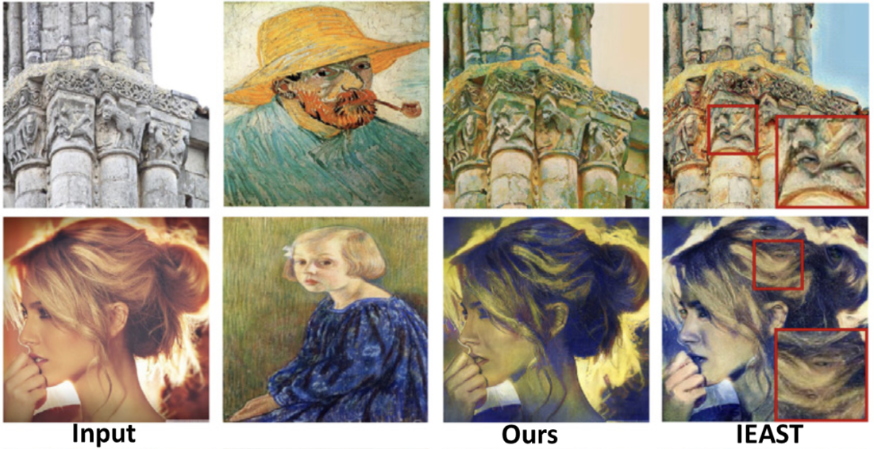
\includegraphics[width=\linewidth]{pics/pic_3.1.1}
%     \caption{\label{fig:pic_3.1.1}三种方法在计算上的差别示意图}
% \end{figure}
% aaa
% \begin{figure}[htbp]
%     \centering
%     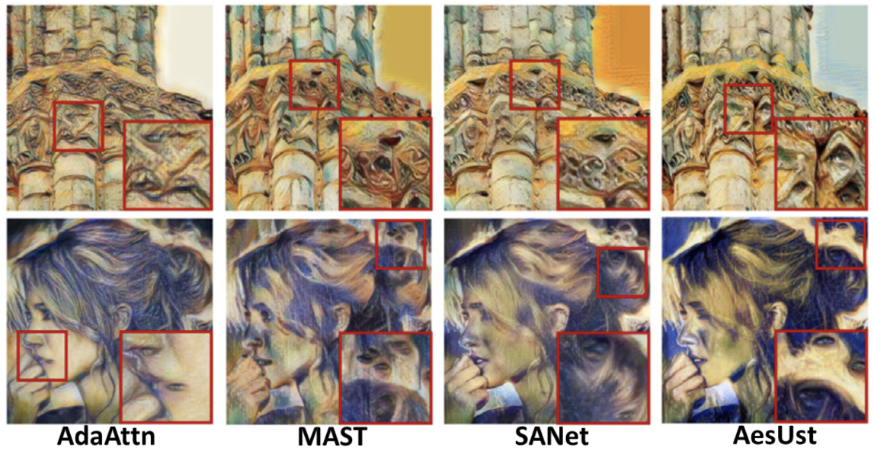
\includegraphics[width=\linewidth]{pics/pic_3.1.2}
%     \caption{\label{fig:pic_3.1.2}三种方法在计算上的差别示意图}
% \end{figure}

% t_n

\begin{equation}
    \label{equ:nerf_color_predict}
    C^{p\text{redict}}(\mathbf{r})=\int_{t_n}^{t_f}T(t)\sigma(\mathbf{r}(t))\mathbf{c}(\mathbf{r}(t),\mathbf{d})dt
\end{equation}
其中$t_n$和$t_f$分别代表相机光线的近界和远界,$\mathbf{r}(t)=o+td$表示光线,$\sigma(t)$表示t处的密度,$\mathbf{c}(\mathbf{r}(t),\mathbf{d})$表示在$\mathbf{r}(t)$处以视角d看过去的颜色值,
$T(t)=\exp{(-\int_{t_n}^t\sigma(\mathbf{r}(s))ds)}$表示t处的不透明度。














% 我们可以用includegraphics来插入现有的jpg等格式的图片,
% 如\autoref{fig:zju-logo}所示。

% \begin{figure}[htbp]
%     \centering
%     
\includegraphics[width=.3\linewidth]{logo/zju}
%     \caption{\label{fig:zju-logo}浙江大学LOGO}
% \end{figure}





% \par 如\autoref{tab:sample}所示,这是一张自动调节列宽的表格。

\begin{table}[htbp]
    \caption{\label{tab:sample}自动调节列宽的表格}
    \begin{tabularx}{\linewidth}{c|X<{\centering}}
        \hline
        第一列 & 第二列 \\ \hline
        xxx & xxx \\ \hline
        xxx & xxx \\ \hline
        xxx & xxx \\ \hline
    \end{tabularx}
\end{table}



\chapter{另一章}


\begin{figure}[htbp]
    \centering
    \includegraphics[width=.3\linewidth]{example-image-a}
    \caption{\label{fig:fig-placeholder}图片占位符}
\end{figure}

\chapter{再一章}

\par 如\autoref{alg:sample},这是一个算法

\begin{algorithm}[H]
    \begin{algorithmic} % enter the algorithmic environment
        \REQUIRE $n \geq 0 \vee x \neq 0$
        \ENSURE $y = x^n$
        \STATE $y \Leftarrow 1$
        \IF{$n < 0$}
            \STATE $X \Leftarrow 1 / x$
            \STATE $N \Leftarrow -n$
        \ELSE
            \STATE $X \Leftarrow x$
            \STATE $N \Leftarrow n$
        \ENDIF
        \WHILE{$N \neq 0$}
            \IF{$N$ is even}
                \STATE $X \Leftarrow X \times X$
                \STATE $N \Leftarrow N / 2$
            \ELSE[$N$ is odd]
                \STATE $y \Leftarrow y \times X$
                \STATE $N \Leftarrow N - 1$
            \ENDIF
        \ENDWHILE
    \end{algorithmic}
    \caption{\label{alg:sample}算法样例}
\end{algorithm}